
\chapter[Thang sóng điện từ]{Thang sóng điện từ}
\section{Lý thuyết}
\subsection {Tổng quát về sóng điện từ}
\begin{itemize}
	\item Thang sóng điện từ là tập hợp các loại sóng điện từ được sắp xếp theo thứ tự bước sóng tăng (tần số giảm) dần.
	\item Các sóng điện từ trong thang sóng điện từ có tần số khác nhau nên tính chất và công dụng của chúng cũng khác nhau.
\end{itemize}
\subsection{Phân loại các sóng điện từ}
\begin{longtable}{|m{4cm}|m{4cm}|m{4cm}|}
	\hline
	\thead{Miền sóng điện từ} 	& \thead{Bước sóng (m)} & \thead{Tần số (Hz)} \\
	\hline
	Sóng vô tuyến điện & $3 \cdot 10^4 \div 10^{-4}$ & $\thicksim 10^4 \div 3 \cdot 10^{12} $  \\
	\hline
	Tia hồng ngoại & $10^{-3} \div \text{7,6} \cdot 10^{-7}$ &  $3 \cdot 10^{11} \div 4 \cdot 10^{14}$\\
	\hline
	Ánh sáng nhìn thấy & $\text{7,6}\cdot 10^{-7} \div \text{3,8} \cdot 10^{-7}$  & $4\cdot 10^{14} \div 8 \cdot 10^{14}$  \\
	\hline	
	Tia tử ngoại	&$\text{3,8} \cdot 10^{-7} \div 10^{-9}$    & $8\cdot 10^{14} \div 3 \cdot 10^{17}$    \\
	\hline
	Tia X & $10^{-8} \div 10^{-11}$& 	$3\cdot 10^{16} \div 3 \cdot 10^{19}$    \\
	\hline
	Tia gamma & 	Dưới $10^{-11}$ & Trên $3 \cdot 10^{19}$ \\
	\hline 
\end{longtable}

\begin{center}
	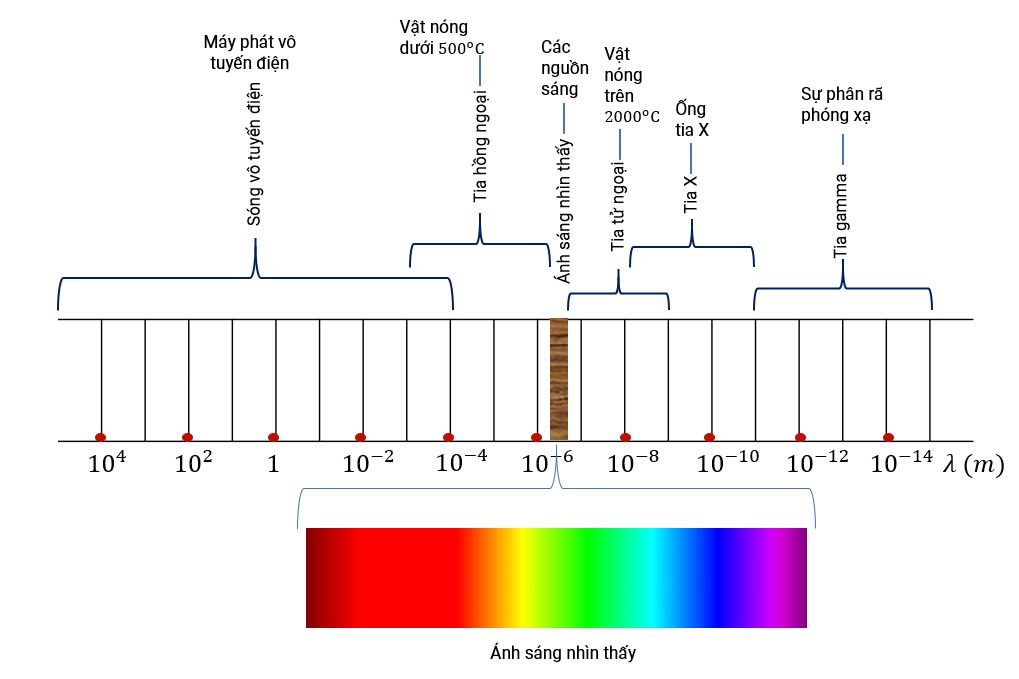
\includegraphics[scale=0.65]{../figs/VN12-PH-36-L-021-6-1.JPG}
\end{center}
\section{Bài tập tự luyện}
\begin{enumerate}[label=\bfseries Câu \arabic*:]
	
	%=======================================
	\item \mkstar{1} [2]
	\cauhoi
	{Với $\varepsilon_{1}, \varepsilon_{2}, \varepsilon_{3}$ lần lượt là photon ứng với các bức xạ màu vàng, bức xạ tử ngoại và bức xạ hồng ngoại thì
		\begin{mcq}(4)
			\item $\varepsilon_{2} > \varepsilon_{3} > \varepsilon_{1}$. 
			\item $\varepsilon_{1} > \varepsilon_{2} > \varepsilon_{3}$. 
			\item $\varepsilon_{3} > \varepsilon_{1} > \varepsilon_{2}$. 
			\item $\varepsilon_{2} > \varepsilon_{1} > \varepsilon_{3}$. 
		\end{mcq}
	}
	
	\loigiai
	{		\textbf{Đáp án: D.}
		
		Năng lượng photon của bức xạ tử ngoại mạnh hơn bức xạ màu vàng và mạnh hơn bức xạ hồng ngoại.
	}
	
	%=======================================
	\item \mkstar{1} [10]
	\cauhoi
	{Trong các loại tia Rơnghen, hồng ngoại, tử ngoại, đơn sắc màu lục, tia có tần số nhỏ nhất là 
		\begin{mcq}(2)
			\item tia tử ngoại. 
			\item tia hồng ngoại. 
			\item tia đơn sắc màu lục. 
			\item tia Rơnghen. 
		\end{mcq}
	}
	
	\loigiai
	{		\textbf{Đáp án: B.}
		
		Tia có tần số nhỏ nhất là tia hồng ngoại.
	}
	
	%=======================================
	\item \mkstar{1} [12]
	\cauhoi
	{Tia hồng ngoại, tia tử ngoại, tia X có tần số lần lượt là $f_{1}, f_{2}, f_{3}$. Sắp xếp theo đúng thứ tự giảm dần là
		\begin{mcq}(4)
			\item $f_{2}, f_{1}, f_{3}$. 
			\item $f_{3}, f_{1}, f_{2}$. 
			\item $f_{2}, f_{3}, f_{1}$. 
			\item $f_{3}, f_{2}, f_{1}$. 
		\end{mcq}
	}
	
	\loigiai
	{		\textbf{Đáp án: D.}
		
		Sắp xếp theo thứ tự tần số giảm dần là: tia X. tia tử ngoại, tia hồng ngoại.
	}
	
	%=======================================
	\item \mkstar{1} [7]
	\cauhoi
	{Các bức xạ được sắp xếp theo thứ tự bước sóng tăng dần là
		\begin{mcq}(1)
			\item ánh sáng tím, tia hồng ngoại, tia tử ngoại, tia X. 
			\item tia X, tia tử ngoại, ánh sáng tím, tia hồng ngoại. 
			\item tia hồng ngoại, ánh sáng tím, tia tử ngoại, tia X. 
			\item tia hồng ngoại, ánh sáng đỏ, tia tử ngoại, tia X. 
		\end{mcq}
	}
	
	\loigiai
	{		\textbf{Đáp án: B.}
		
		Sắp xếp theo thứ tự tăng dần bước sóng là tia X, tia tử ngoại, ánh sáng tím, tia hồng ngoại.
	}
	
	
\end{enumerate}

